\documentclass[11pt, a4paper]{article}

% --- PAQUETES DE CONFIGURACIÓN BÁSICA ---
\usepackage[utf8]{inputenc}
\usepackage[T1]{fontenc}
\usepackage[spanish, es-nodecimaldot]{babel}
\usepackage{graphicx}
\usepackage[top=2.2cm, bottom=2.5cm, left=2.2cm, right=2.2cm]{geometry}
\usepackage{caption}
\usepackage{float}
\usepackage{microtype}
\usepackage{booktabs}
\usepackage{amsmath}
\usepackage{xcolor}
\usepackage{tabularx}
\usepackage[colorlinks=true, linkcolor=blue!70!black, urlcolor=blue!70!black, citecolor=blue!70!black]{hyperref}

% Rutas de búsqueda para figuras
\graphicspath{{output/figures/}{figures/}{output/docx_images/}{./}}

% Configuración de títulos y figuras
\captionsetup{font=small, labelfont=bf, justification=centering}

\title{\textbf{Trabajo Práctico 5: Medio Ambiente, Instituciones y Desarrollo}\\[0.3em]
\large Evidencia Empírica para la India (1960--2025)}
\author{
    \small \textbf{Mateo Barros} \quad \textbf{Felipe Delgado} \quad \textbf{Santiago González} \quad \textbf{Rodrigo Stremel} \quad \textbf{Santiago Trivellini} \\[0.3em]
    \small \textit{Desarrollo Económico --- Licenciatura en Economía --- Universidad Nacional del Sur (UNS)}
}
\date{\small Septiembre de 2026}

\begin{document}

\maketitle

\vspace{-1em}
\noindent\rule{\textwidth}{0.6pt}
\vspace{0.8em}

\section{Parte 1: Instituciones y Desarrollo}

\subsection{Análisis Descriptivo de las Series Institucionales}

La evolución de los indicadores de gobernabilidad es más bien poco uniforme. No se observa ninguna tendencia clara en la mayoría de indicadores: o son de alta volatilidad, o están estancados en el mismo nivel de 1996. Los que parecen seguir el casi lineal movimiento positivo del PIB son la eficacia del gobierno (calidad de los servicios públicos, calidad de la función pública y credibilidad institucional), y la estabilidad política (aunque sigue en niveles negativos comparando a la media mundial). El indicador de gobernabilidad general (promedio simple de cada dimensión) sí tiende a seguir la tendencia del PIB, con ciclos de auge y caídas.

\begin{figure}[H]
    \centering
    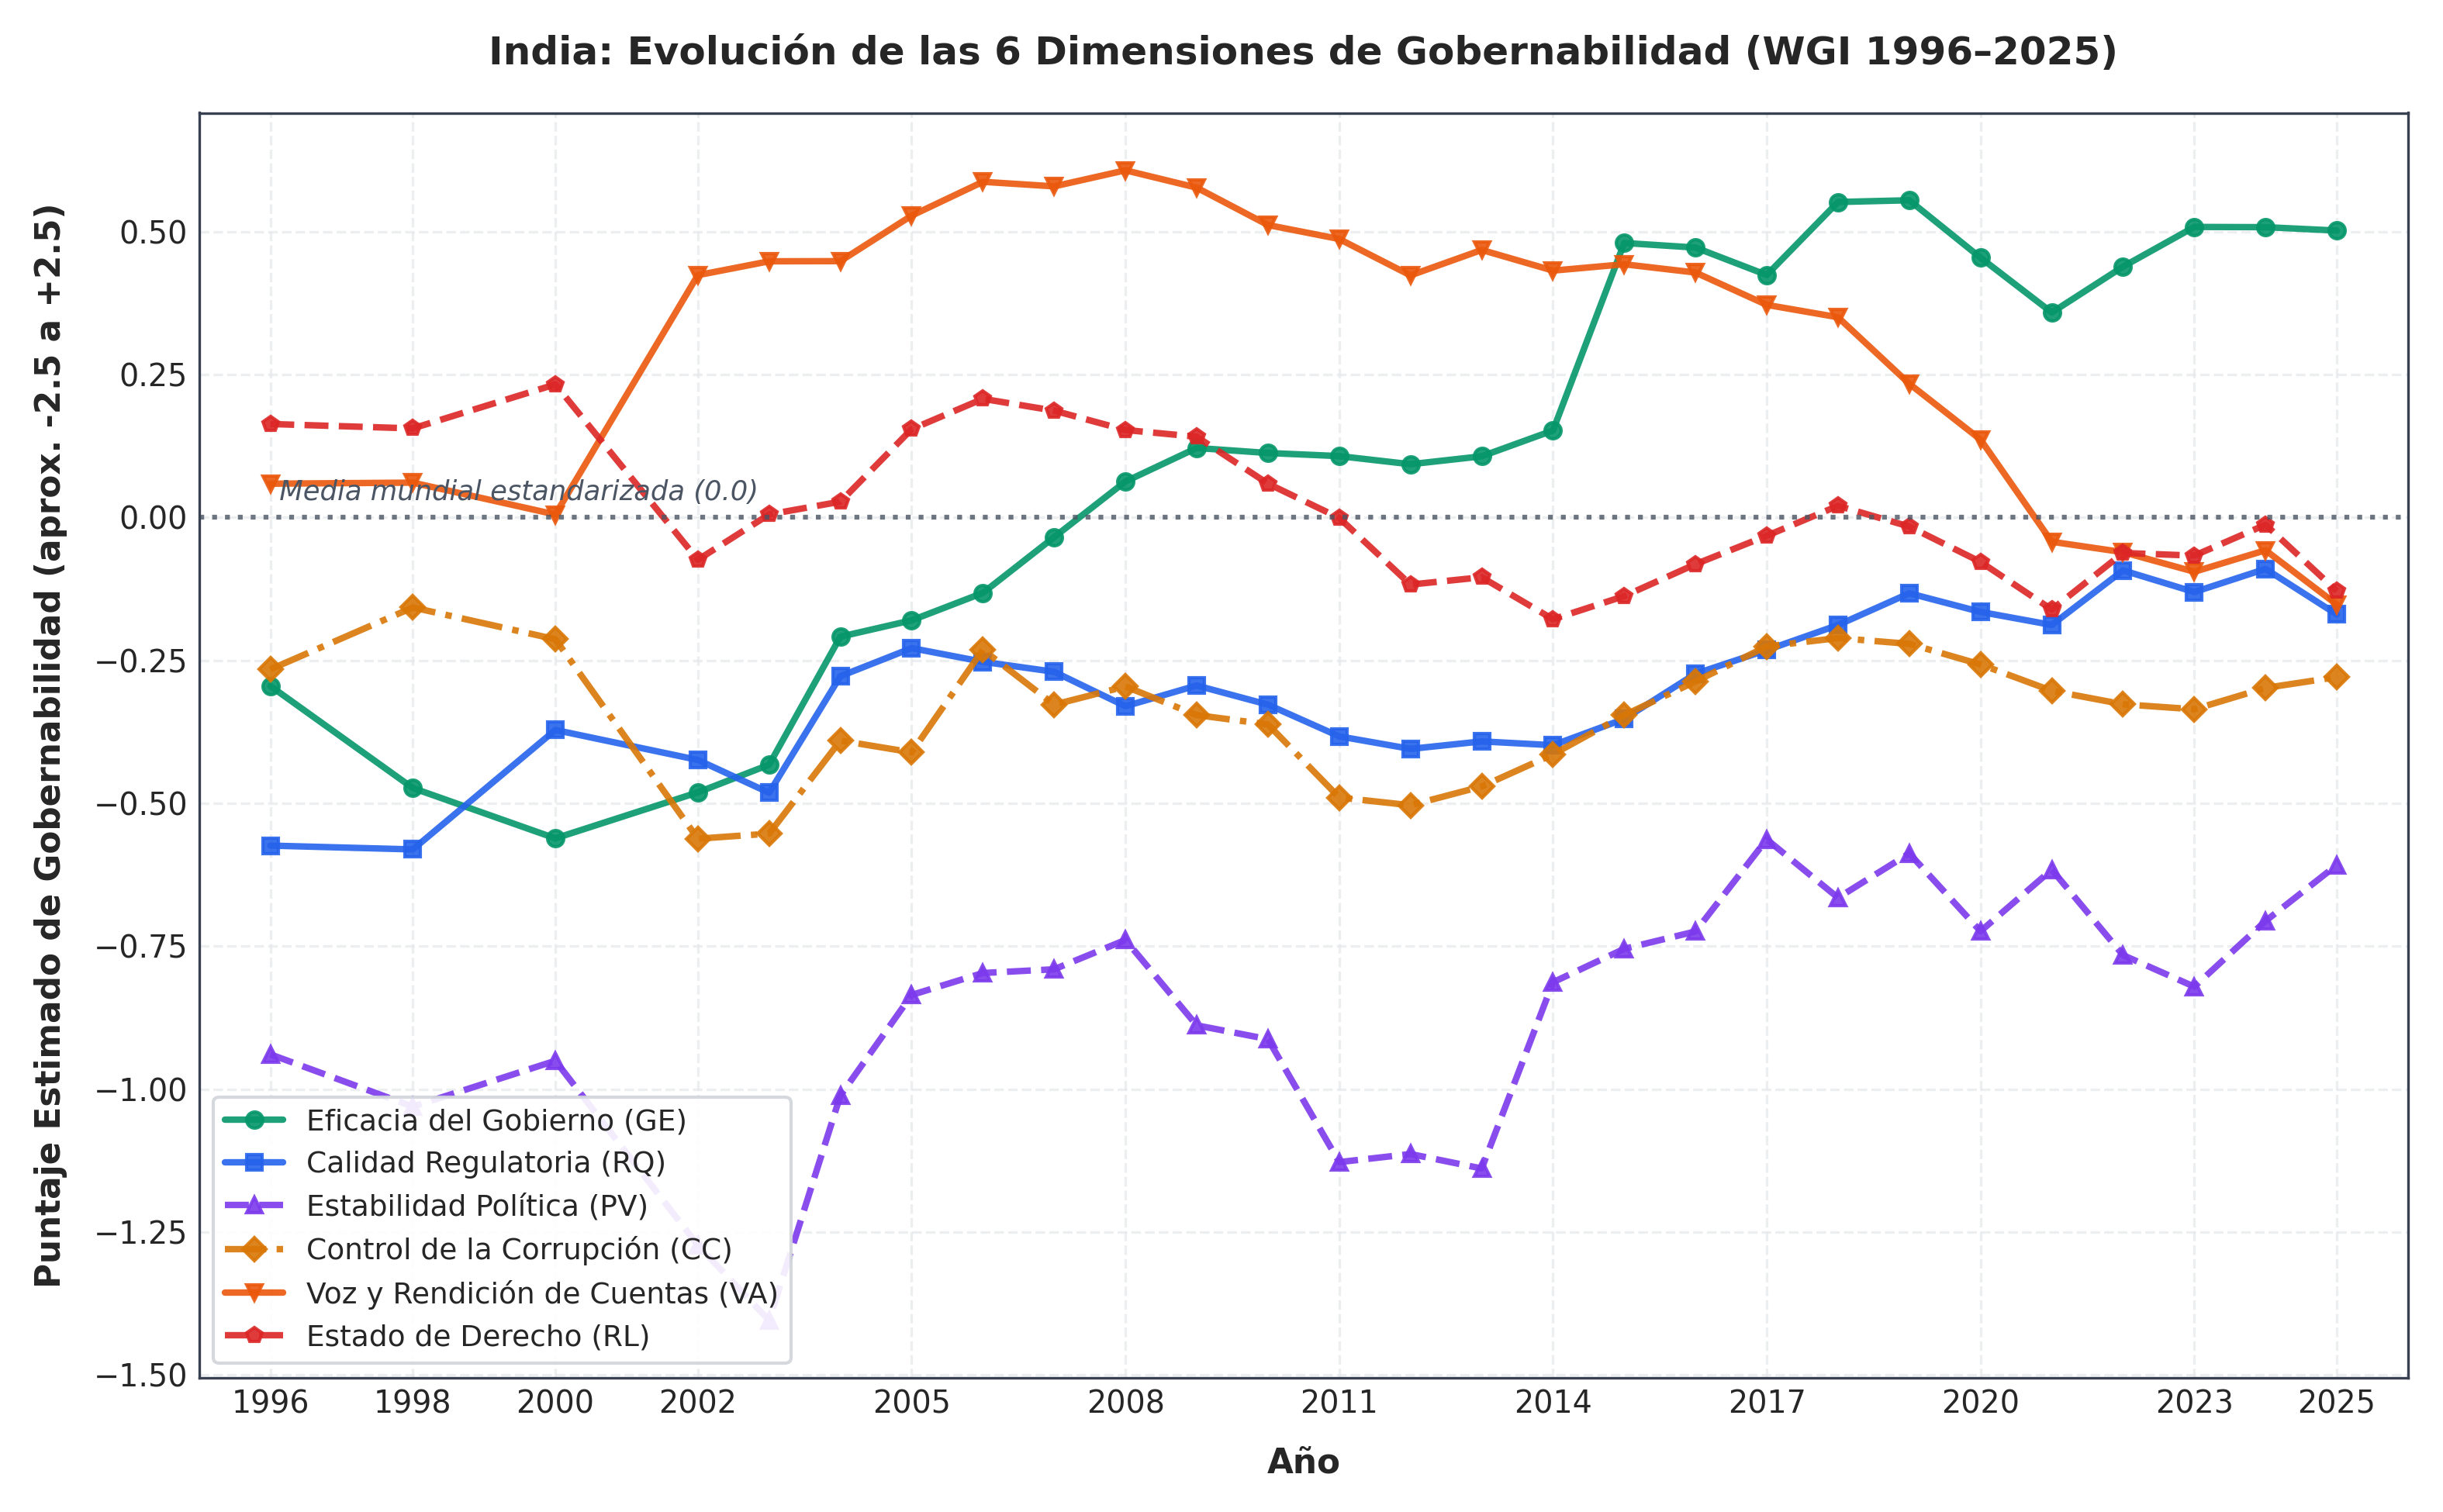
\includegraphics[width=0.92\textwidth]{grafico1_wgi_series_temporales.png}
    \caption{\textbf{India: Evolución de las 6 Dimensiones de Gobernabilidad (WGI 1996--2025).} \\
    Fuente: Worldwide Governance Indicators, World Bank.}
    \label{fig:wgi_series}
\end{figure}

\begin{figure}[H]
    \centering
    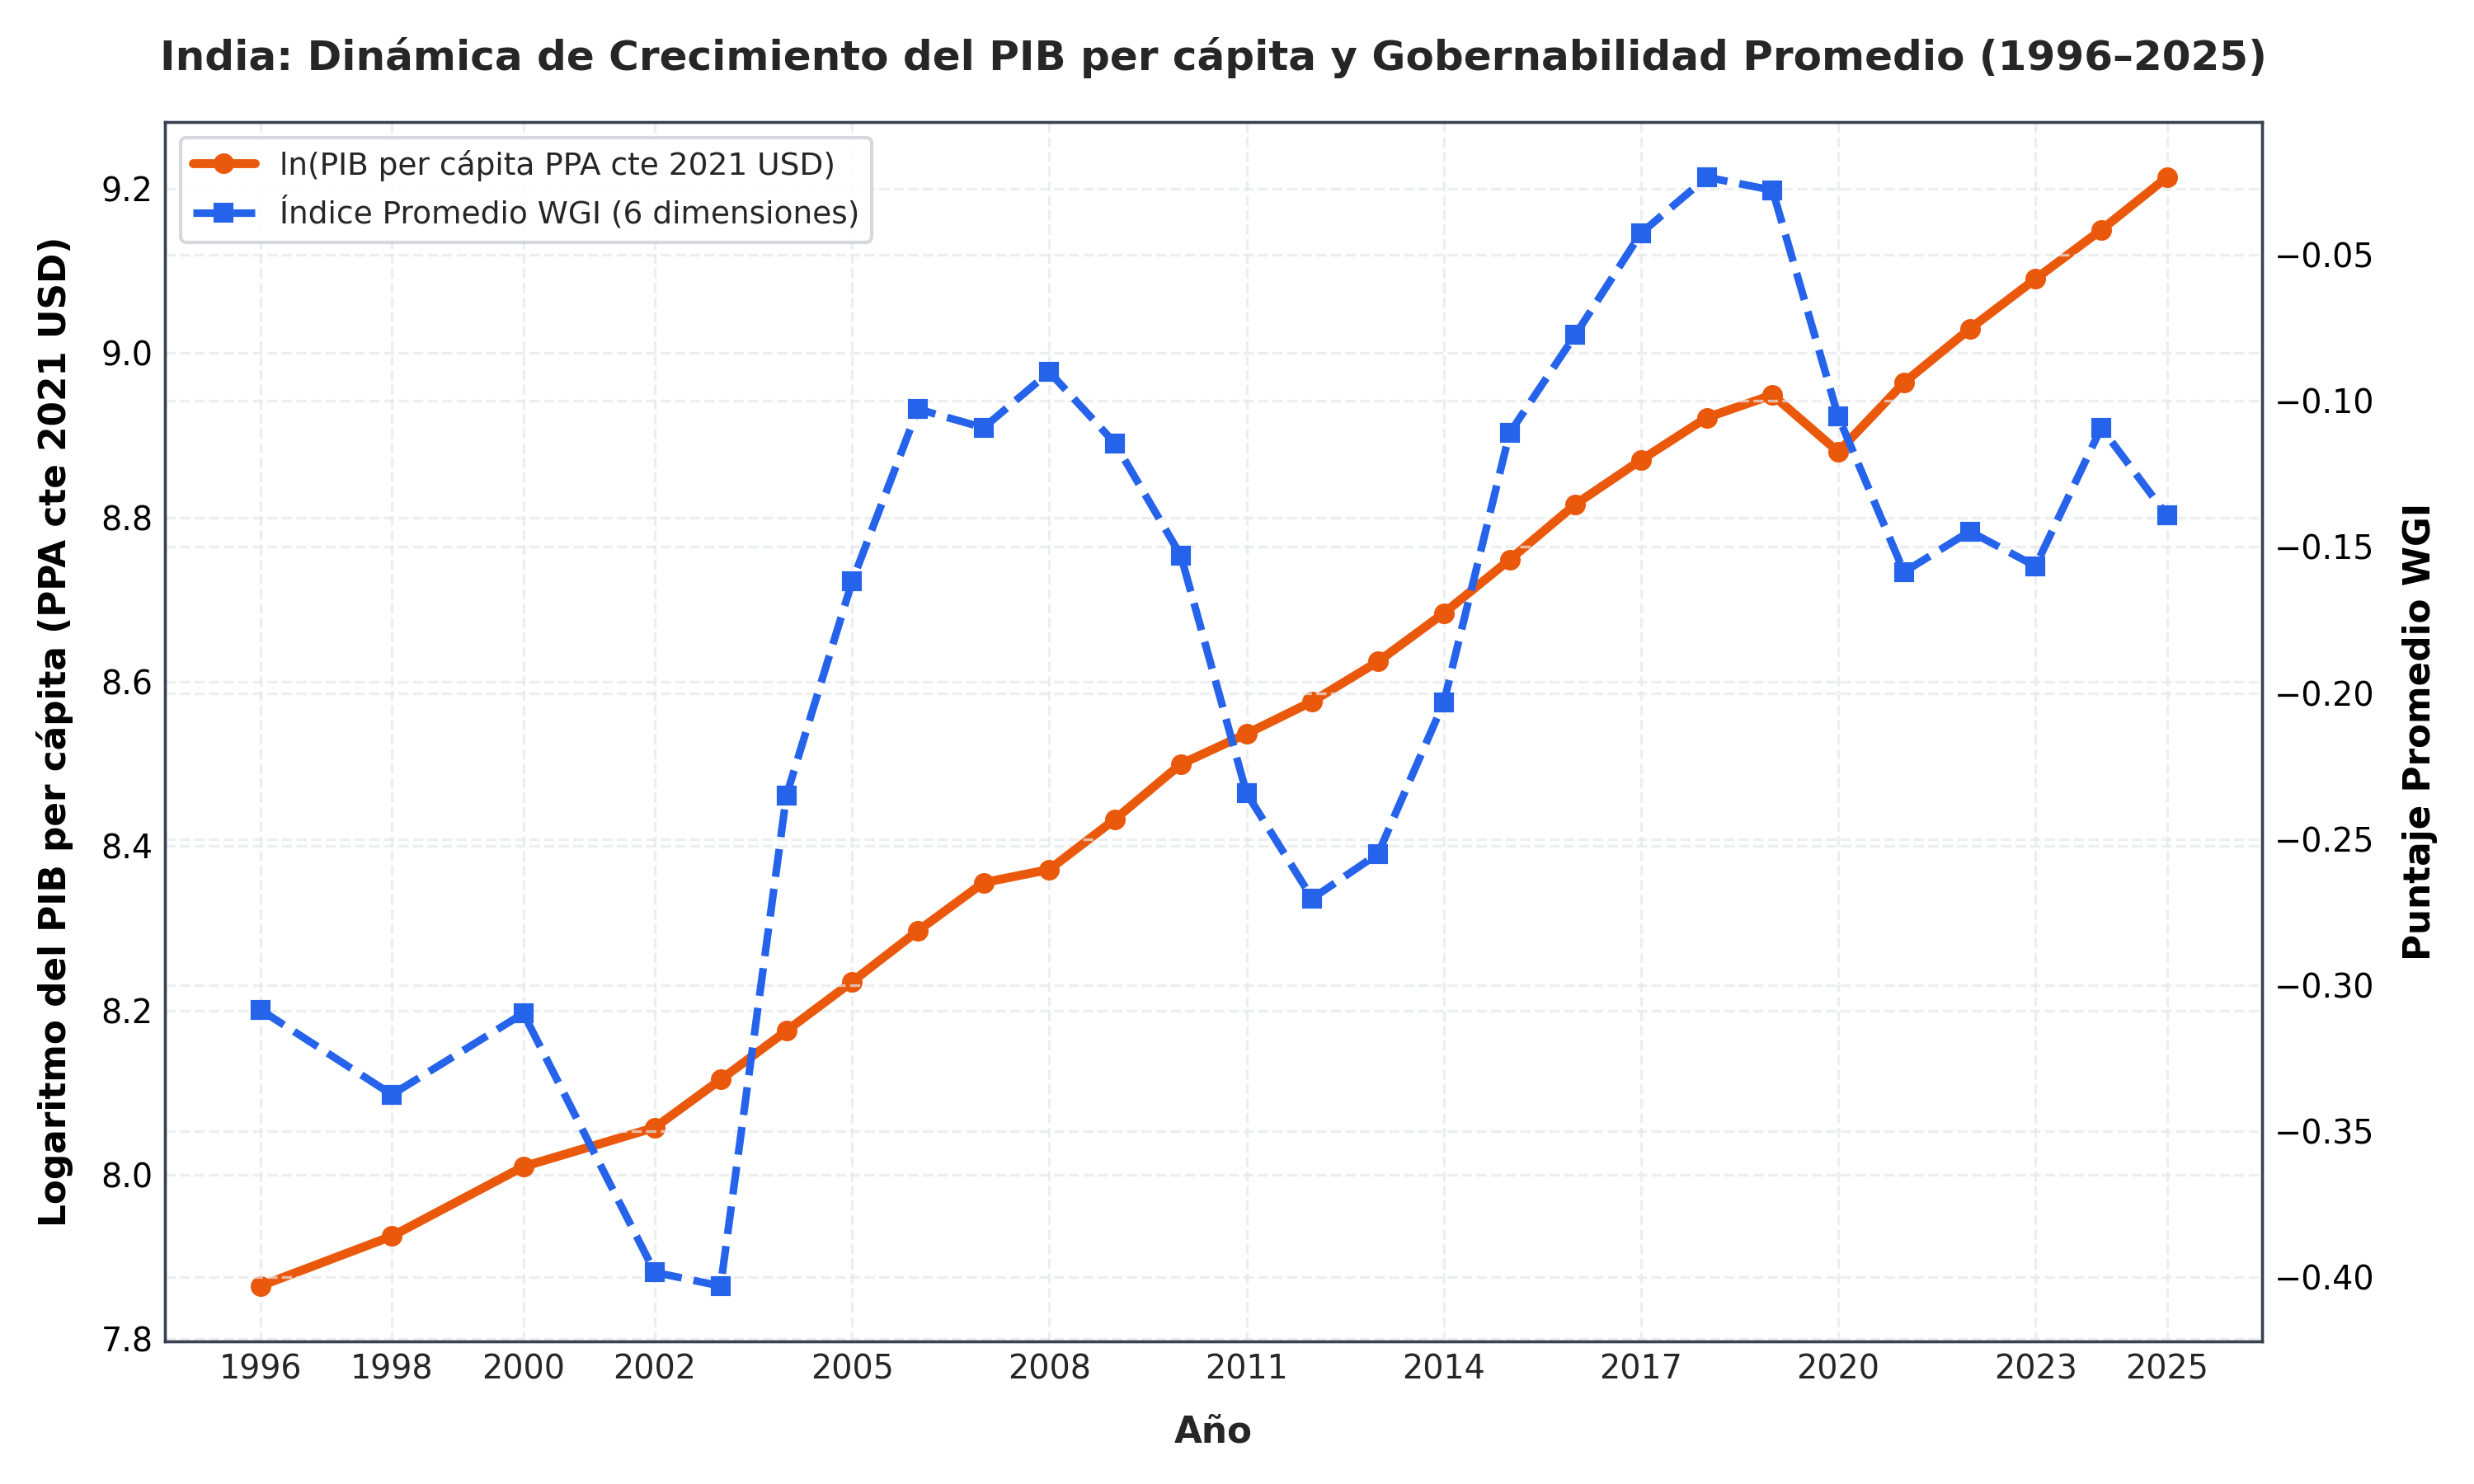
\includegraphics[width=0.92\textwidth]{grafico2_pib_vs_gobernabilidad_promedio.png}
    \caption{\textbf{India: Dinámica de Crecimiento del PIB per cápita y Gobernabilidad Promedio (1996--2025).} \\
    Fuente: WGI y World Development Indicators, World Bank.}
    \label{fig:pib_wgi_prom}
\end{figure}

\newpage
\subsection{Estimación MCO}

Para la regresión, como variables de control elegimos a la apertura económica (dinámica clave en el proceso de políticas iniciado en los años noventa) y el gasto en educación como porcentaje del PIB.

\begin{table}[H]
\centering
\caption{\textbf{Instituciones y Controles Macro}}
\label{tab:stata_regression}
\resizebox{\textwidth}{!}{%
\begin{tabular}{lccccc}
\toprule
\textbf{Variable} & \textbf{Coeficiente ($\hat{\beta}$)} & \textbf{Std. Err.} & \textbf{$t$-stat} & \textbf{$P > |t|$} & \textbf{[95\% Conf. Interval]} \\
\midrule
Voz y Rendición de Cuentas (\texttt{va}) & $-0.2425^{***}$ & $0.0813$ & $-2.98$ & $0.008$ & $[-0.4134,\; -0.0717]$ \\
Estabilidad Política (\texttt{pv})        & $-0.1111$       & $0.1763$ & $-0.63$ & $0.537$ & $[-0.4815,\; \phantom{-}0.2593]$ \\
Eficacia del Gobierno (\texttt{ge})       & $\phantom{-}0.5806^{***}$  & $0.1043$ & $\phantom{-}5.57$  & $0.000$ & $[\phantom{-}0.3616,\; \phantom{-}0.7997]$ \\
Calidad Regulatoria (\texttt{rq})         & $\phantom{-}0.7178^{***}$  & $0.1919$ & $\phantom{-}3.74$  & $0.001$ & $[\phantom{-}0.3146,\; \phantom{-}1.1210]$ \\
Estado de Derecho (\texttt{rl})           & $-0.6017^{**}$  & $0.2762$ & $-2.18$ & $0.043$ & $[-1.1819,\; -0.0215]$ \\
Control de la Corrupción (\texttt{cc})    & $\phantom{-}0.2026$       & $0.3589$ & $\phantom{-}0.56$  & $0.579$ & $[-0.5515,\; \phantom{-}0.9566]$ \\
Apertura Comercial (\texttt{aper\_comerc})& $\phantom{-}0.0075^{***}$  & $0.0024$ & $\phantom{-}3.19$  & $0.005$ & $[\phantom{-}0.0026,\; \phantom{-}0.0125]$ \\
Gasto Educación (\texttt{gasto\_educ\_interp}) & $\phantom{-}0.0526$  & $0.0569$ & $\phantom{-}0.92$  & $0.368$ & $[-0.0669,\; \phantom{-}0.1721]$ \\
Constante (\texttt{\_cons})               & $\phantom{-}6.8631^{***}$  & $0.2925$ & $23.46$  & $0.000$ & $[\phantom{-}6.2485,\; \phantom{-}7.4777]$ \\
\midrule
\multicolumn{6}{l}{\footnotesize $N = 27$ observaciones (1996--2025) \quad $R^2 = 0.9818$ \quad $R^2 \text{ ajustado} = 0.9737$ \quad $F(8, 18) = 121.36^{***}$} \\
\bottomrule
\end{tabular}%
}
\begin{minipage}{\textwidth}
\vspace{0.3em}
\scriptsize \textit{Nota:} Variable dependiente: $\ln(\text{PIBpc})$. Estimación en base a salida de Stata. $^{***}\ p<0.01$, $^{**}\ p<0.05$, $^{*}\ p<0.10$.
\end{minipage}
\end{table}

\subsection{Interpretación}

Las dimensiones significativas fueron la Voz y Rendición de Cuentas (participación ciudadana y derechos civiles), la Eficacia del Gobierno, la Calidad Regulatoria y el Estado de Derecho (confianza y cumplimientos de las normas de la sociedad).

Las variables no significativas no corresponden a una no-correlación con el crecimiento, sino que su alto $p$-value se debe a la existencia de colinealidad con el resto de dimensiones. Si se regresa un modelo con cada una de las variables por separado sí se demuestra relación (ver anexo). La dimensión con mayor efecto sobre el PIB es la calidad regulatoria: su estimador de 0,71 indica que un aumento de 0,1 puntos en dicha variable implica un aumento de 7\% en el PIB per cápita.

El resto de variables significativas, incluyendo la apertura comercial, muestra el signo esperado (positivo). Sin embargo, la dimensión de Estado de Derecho señala significancia estadística y una relación inversa con el movimiento del producto. Un aumento de 0,1 puntos en dicho indicador implica una disminución aproximada del 6\% en el PIB. Asimismo, el coeficiente de Voz y Rendición tampoco presenta el signo esperado: un aumento de 0,1 puntos del indicador genera una caída del 2,5\% en el PIB.

Este fenómeno puede explicarse a través del ``Dilema de los Países en Desarrollo''. En la India, la velocidad del crecimiento de los mercados ha superado crónicamente la capacidad de adaptación de un sistema judicial (Estado de Derecho) y la capacidad de formalizar su economía (Voz y Rendición). Al ser una economía embebida en la flexibilidad e informalidad es posible que las reformas estatales sean interpretadas por los agentes como rigideces normativas. Este signo inverso halla consistencia con la tesis de Acemoglu y Robinson, quienes reconocen que las economías emergentes pueden experimentar períodos de expansión acelerada bajo configuraciones institucionales débiles o extractivas, donde la imposición prematura o rígida de un marco legal altera las dinámicas de acumulación y los acuerdos que sostienen el dinamismo del producto en el corto plazo.

\vspace{0.5em}
\noindent\rule{\textwidth}{0.6pt}
\vspace{0.5em}

\section{Parte 2: Medio Ambiente y Desarrollo}

\subsection{Conceptos: Huella Ecológica y Biocapacidad}
La ``huella ecológica'' mide la demanda y la oferta de la naturaleza. Es una métrica que mide cuánta naturaleza tenemos como sociedad y cuánta naturaleza utilizamos periódicamente:
\begin{itemize}
    \item \textbf{Demanda:} Suma las áreas biológicamente productivas y mide los recursos ecológicos que una población o producto necesita para producir el recurso natural que consume y para absorber sus residuos (emisiones de carbono).
    \item \textbf{Oferta:} Es justamente la biocapacidad de una ciudad, estado o nación que representa la productividad de sus recursos ecológicos. Áreas que, si no se explotan, también absorben residuos que generamos.
\end{itemize}

La biocapacidad es la capacidad de los ecosistemas para producir materiales biológicos utilizados por las personas y para absorber los residuos generados por los seres humanos, bajo los esquemas de gestión y las tecnologías de extracción actuales. La biocapacidad puede variar de un año a otro debido al clima, la gestión y la proporción considerada como insumos útiles para la economía humana.

Es importante tener en cuenta que la huella ecológica y la biocapacidad se expresan en hectáreas globales (\textit{gha}), comparables a nivel mundial con la productividad media mundial.

Tal como nos cuenta desde hace tiempo la ley de oferta y demanda, si la huella ecológica supera la biocapacidad, nos encontramos ante un déficit de esta última. Esto es lo que sucede en el caso de India, con un -200\% de magnitud de exceso de huella ecológica por sobre la biocapacidad india.

Es decir, la demanda de bienes y servicios (de la sociedad) que la tierra y mares proporcionan (oferta) excede la capacidad de regeneración de los ecosistemas de la región, representando un caso perjudicial para futuras generaciones en términos de sustentabilidad. Este exceso de demanda se satisface agotando sus propios recursos y emitiendo dióxido de carbono a la atmósfera o, en última instancia, con importaciones.

En el caso contrario, y debiendo representar el objetivo de las sociedades, si la biocapacidad superara su Huella, se poseería una reserva de biocapacidad.

\begin{figure}[H]
    \centering
    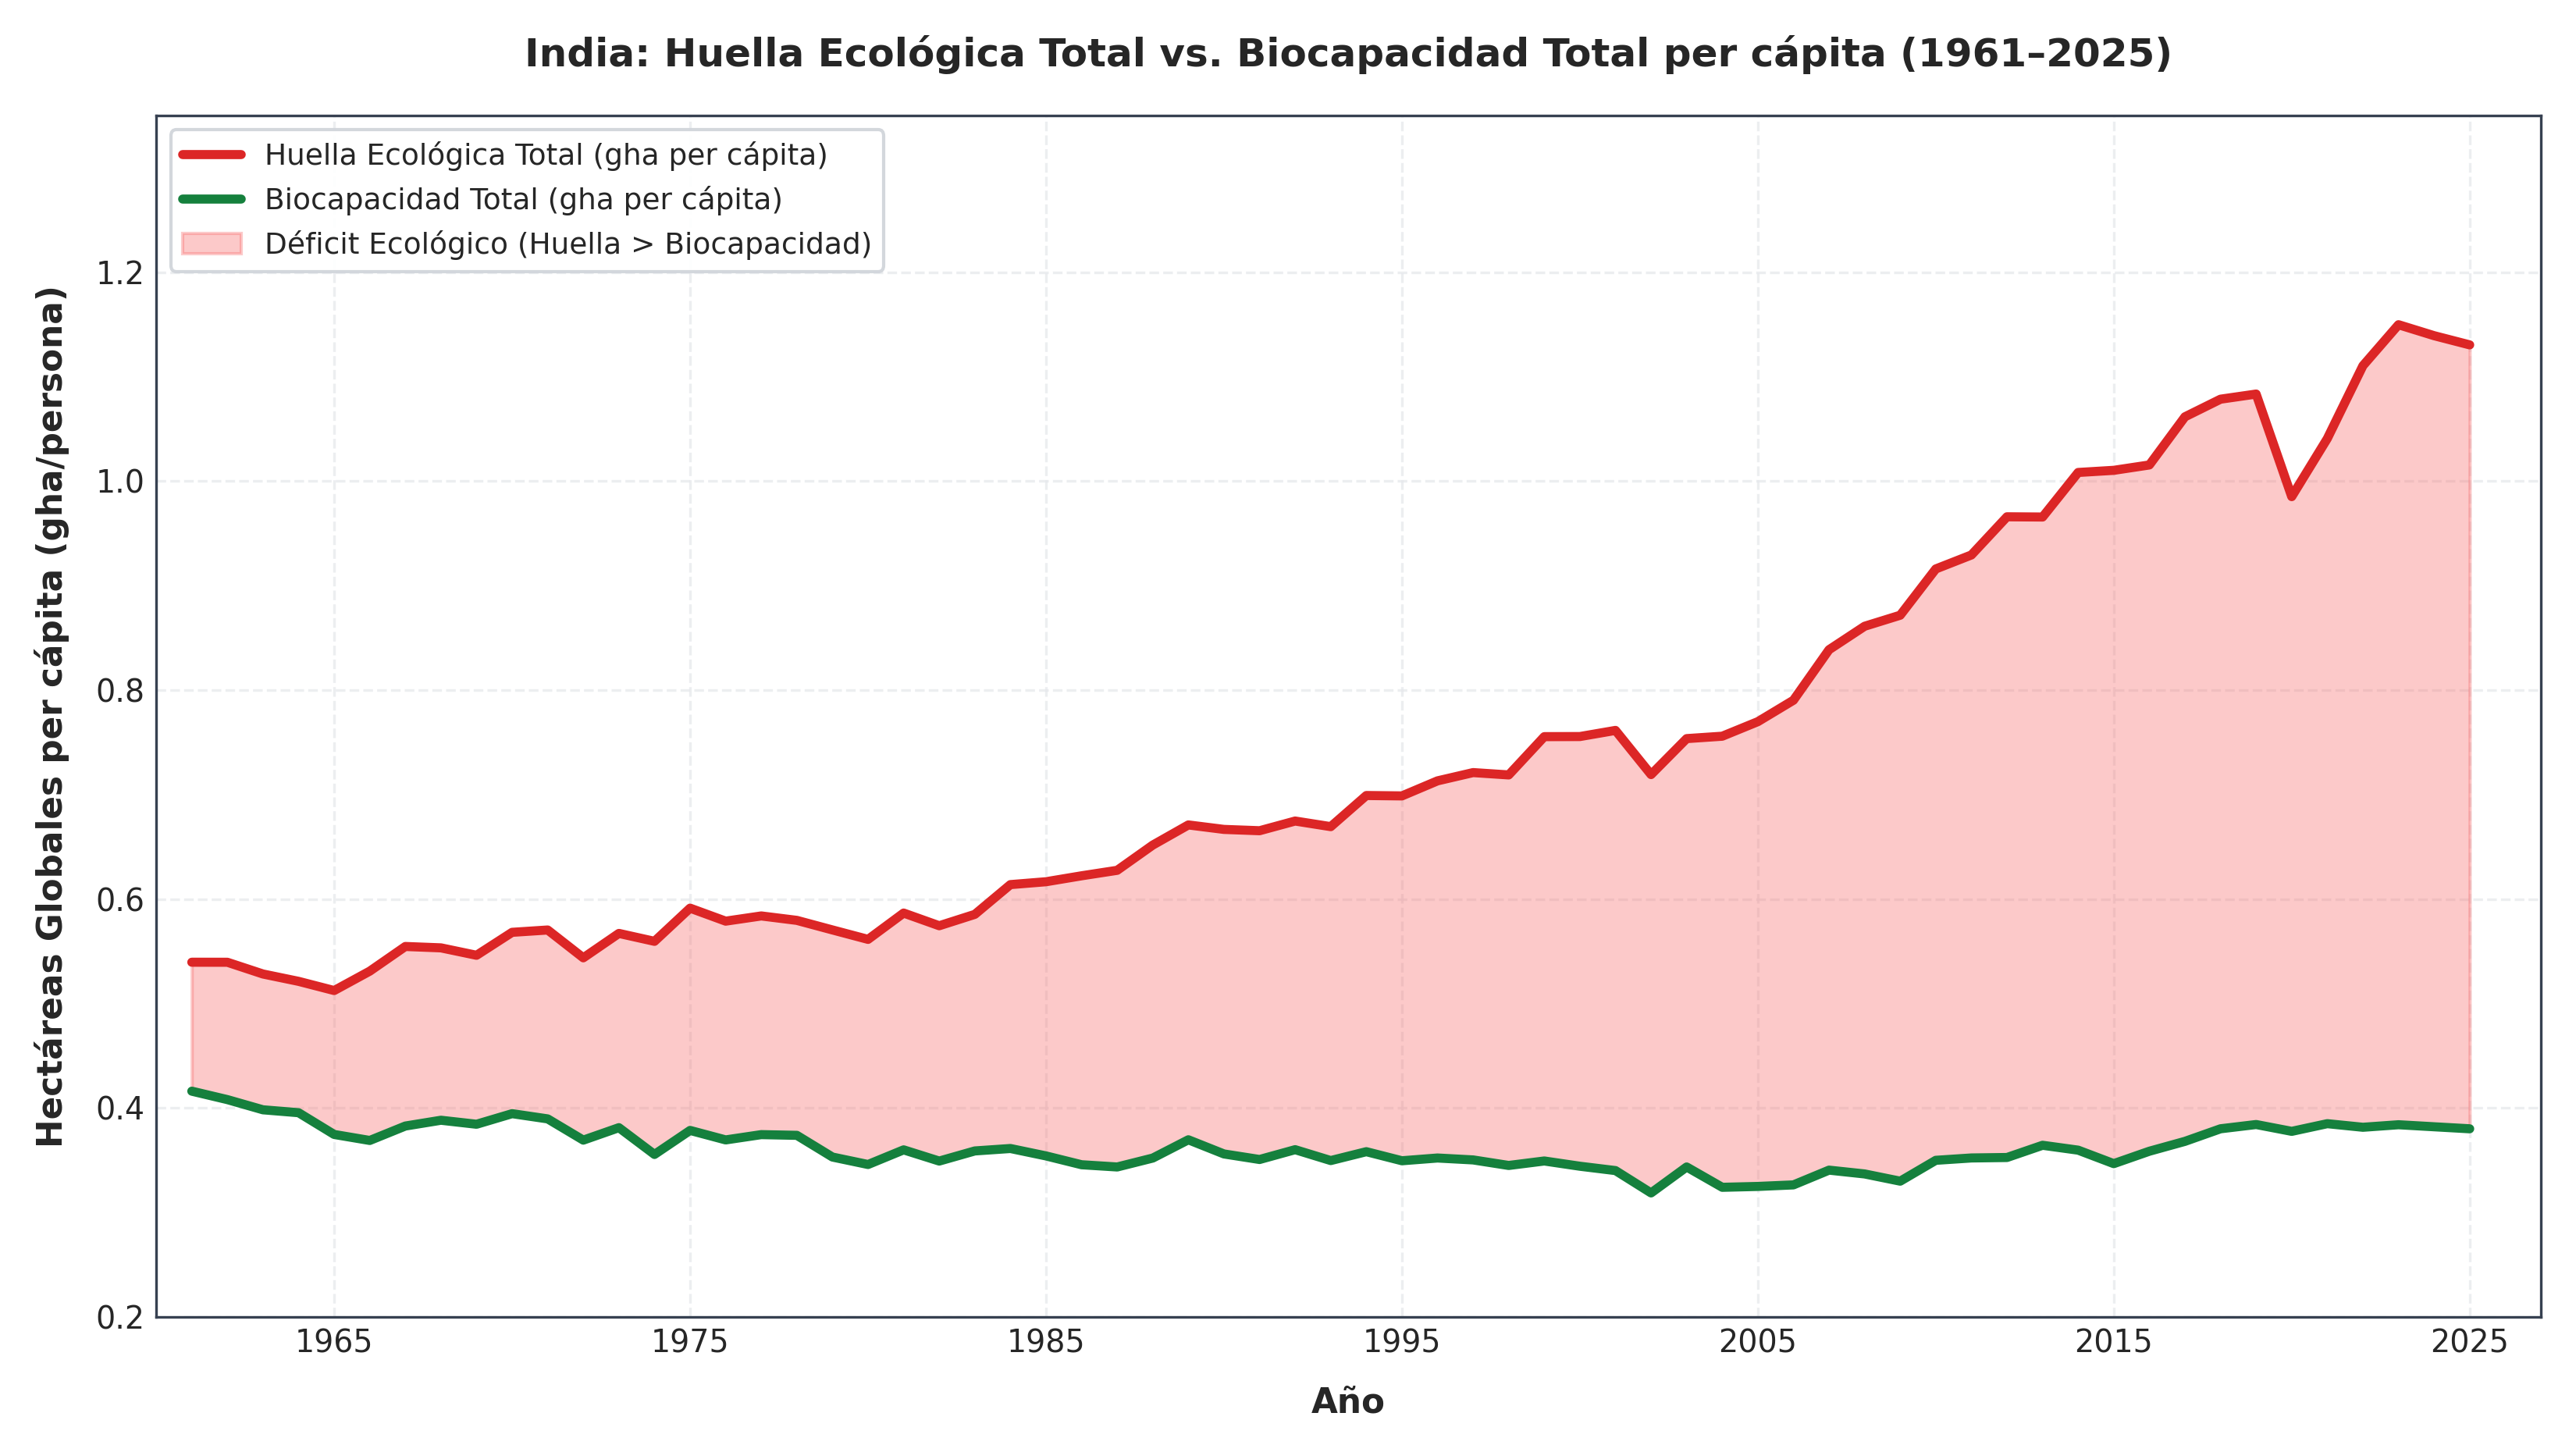
\includegraphics[width=0.92\textwidth]{grafico5_huella_ecologica_vs_biocapacidad.png}
    \caption{\textbf{India: Huella Ecológica Total vs. Biocapacidad Total per cápita (1961--2025).} \\
    Fuente: National Footprint and Biocapacity Accounts, Global Footprint Network (GFN).}
    \label{fig:huella_biocapacidad}
\end{figure}

\subsection{Evolución del Balance Ecológico y Causas del Déficit}

Medimos en el gráfico dos variables: la biocapacidad por persona (área productiva, es decir, su ``ingreso ecológico'') y la huella ecológica por persona (áreas biológicamente productivas por persona que necesitan para producir todo lo que consumen).

Tomando el período entre 1960 a la actualidad, se evidencia un continuo déficit ecológico total.

Además, se puede ver cómo a mediados de los 80s, la huella ecológica cambia su tendencia, comenzando con una inclinación creciente, para que luego, a comienzos del siglo, dicha tendencia se abrupte aún más, concordando con el impulso del crecimiento económico que se dio en India en los 90s y la intensificación en la globalización. Por su lado, la biocapacidad per cápita permaneció estancada durante todo el período, explicándose principalmente por la degradación ambiental (quemas, residuos y emisiones, entre otras causas).

La relación entre el aumento en la huella ecológica y la expansión económica se explica por el incremento en la producción y el consumo. Es decir, al aumentar el ingreso, se genera una mayor explotación y consumo de recursos. A la vez, esto trae consigo una ampliación de la urbanización e industrialización.

\begin{figure}[H]
    \centering
    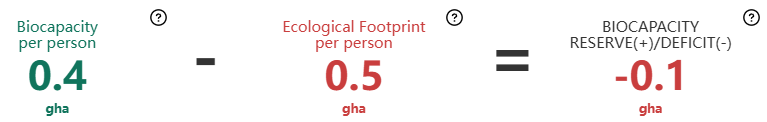
\includegraphics[width=0.75\textwidth]{image1_balance_widget.png}
    \caption{\textbf{Balance Ecológico per cápita: Relación entre Biocapacidad y Huella Ecológica.} \\
    Fuente: Global Footprint Network.}
    \label{fig:widget_balance}
\end{figure}

En datos per cápita del 2024, la biocapacidad es el área productiva que existe por persona en India, restando la huella ecológica por persona da como resultado -0,1.

\newpage
\appendix
\section{Anexo: Regresiones Auxiliares}

Como se mencionó en la sección de estimación, presentamos los resultados de los modelos por separado para evaluar la relación de cada dimensión de gobernabilidad con el PIB per cápita al controlar por apertura comercial y gasto público en educación.

\begin{table}[H]
\centering
\small
\caption{\textbf{Resumen y Resultados (o no) Esperados}}
\label{tab:anexo_sintesis}
\begin{tabular*}{\textwidth}{l @{\extracolsep{\fill}} ccc}
\toprule
\textbf{Variable} & \textbf{Beta ($\hat{\beta}$)} & \textbf{$p$-value} & \textbf{Conclusión del Impacto} \\
\midrule
Voz y Rendición de Cuentas (\texttt{va}) & $-0.4832$ & $0.035^{**}$  & \textbf{Negativa inesperada} (significativa) \\
Estabilidad Política (\texttt{pv})       & $+0.7096$ & $<0.001^{***}$ & \textbf{Positiva esperada} (significativa) \\
Eficacia del Gobierno (\texttt{ge})      & $+0.8160$ & $<0.001^{***}$ & \textbf{Positiva esperada} (la más determinante) \\
Calidad Regulatoria (\texttt{rq})        & $+1.4221$ & $<0.001^{***}$ & \textbf{Positiva esperada} (significativa) \\
Estado de Derecho (\texttt{rl})          & $-0.3806$ & $0.485$        & \textbf{Negativa inesperada} (no significativa) \\
Control de la Corrupción (\texttt{cc})   & $+0.9340$ & $0.025^{**}$   & \textbf{Positiva esperada} (significativa) \\
\midrule
Índice Promedio WGI                      & $+1.5259$ & $<0.001^{***}$ & \textbf{Positiva esperada} (significativa) \\
\bottomrule
\end{tabular*}
\begin{minipage}{\textwidth}
\vspace{0.3em}
\scriptsize \textit{Nota:} Modelos bivariados con controles de apertura comercial y gasto educativo interpolado ($N = 27$). $^{***}\ p<0.01$, $^{**}\ p<0.05$.
\end{minipage}
\end{table}

\end{document}
